\section{Stochastic Processes}
Consider the following game: given a fair coin, you win $1$ if the outcome is \textit{Head} and lose $1$ if the outcome is \textit{Tail}. Without any loss of generality, let's denote head and tail with the numbers $+1$ and $-1$, respectively. Now, tossing the coin three times defines the following sample space 

\begin{equation*}
    \Omega = \Big\{ \omega=(\omega_1, \omega_2, \omega_3) : \omega_i \in \{-1,+1\} \Big\}
\end{equation*}

Let's define three random variables $X_1 = \omega_1, X_2 = \omega_1+\omega_2$ and $X_3 = \omega_1+\omega_2+\omega_3$. Each one of these is describing the total win after each toss, we may think of it as recording the profit/loss as \textit{time} goes by. Tosses are independent, therefore the joint measure of the vector $\omega$ is the product measure $\mathbb{P} = \mathbb{P}_1 \otimes \mathbb{P}_2 \otimes \mathbb{P}_3$. The only element missing to build a proper \textit{probability space}, other than the sample space and the measure, is the $\sigma-$algebra. Many choices are possible, starting from the most obvious one, not to mention the largest, the power set $\mathcal{P}(\Omega)$. We want to follow a different approach: we know every random variable can generate a different $\sigma-$algebra. For instance, let's take the first random variable $X_1$ and work out what's inside of $\sigma(X_1)$. Other than the empty set and the sample space itself, we must include the counter images of every value $X_1$ can assume: namely $X^{-1}(1)$ and $X^{-1}(-1)$. We call these two sets $A_1,A_2$, respectively. 

\begin{gather*}
    A_1 = \Big\{(1,1,1);(1,1,-1);(1,-1,1);(1,-1,-1) \Big\} \;\; A_2 = \Big\{(-1,1,1);(-1,1,-1);(-1,-1,1);(-1,-1,-1) \Big\} \\
    \implies \mathcal{F}_1 = \Big\{\emptyset, \Omega, A_1, A_2 \Big\}
\end{gather*}

Now, compare this to $\sigma(X_1,X_2)$, the $\sigma-$algebra generated by both the first and the second random variable. Again, beside the empty set and the sample set, we shall focus on all the possible counter images. $X_1$ can take two values, while $X_2$ can be equal to either $2,0$ or $-2$. This means we have a total of four different counter sets 

\begin{gather*}
    B_1 = \Big\{ (1,1,1) ; (1,1,-1) \Big\} \;\; B_2 = \Big\{ (1,-1,1); (1,-1,-1) \Big\} \\
    B_3 = \Big\{ (-1,1,1) ; (-1,1,-1) \Big\} \;\;     B_4 = \Big\{ (-1,-1,1) ; (-1,-1,-1) \Big\} \\
    \implies \mathcal{F_2} = \Big\{ \emptyset, \Omega, B_1,B_2,B_3,B_4 \Big\}
\end{gather*}

It's clear that $\mathcal{F}_2$ is far richer than $\mathcal{F}_1$, in fact $\mathcal{F}_1 \subset \mathcal{F}_2$. In other words, the latter contains \textit{more information} with respected to the former. This framework comes into play very often: the flow of information as time passes is described through and increasing family of $\sigma-$algebras. Mathematically, a collection of $\sigma-$algebras $(\mathcal{F}_t)_t$ such that $\mathcal{F}_s \subset \mathcal{F}_t$, for $s \leq t$, is called a \textit{filtration}.

\begin{definition}
    A \textbf{stochastic process} $X$ is an object of the form $X = (\Omega, \mathcal{F}, (\mathcal{F}_t)_t, X_t, \mathbb{P})$ where $t \in T$ is the set of time indexes. Moreover, $(\Omega, \mathcal{F}, \mathbb{P})$ is a probability space, $(\mathcal{F}_t)$ is a filtration and $X_t$ denotes a family of random variables $X_t : (\Omega,\mathcal{F},\mathbb{P}) \to (E,\mathcal{B})$, pointing to a measurable space, such that every single $X_t$ is $\mathcal{F}_t-$measurable. 
\end{definition}

A collection of random variables $X_t$ that satisfies this last cited property is known as $\mathcal{F}_t-$\textit{adapted}. Note that, since we are dealing with a filtration, the fact that $X_s$ is $\mathcal{F}_s-$measurable clearly implies that $X_s$ is also $\mathcal{F}_t-$measurable, for every $s \leq t$, as $\mathcal{F}_s \subset \mathcal{F}_t$. In particular, $\mathcal{F}_t$ contains the $\sigma-$algebra generated by every $X_s$ up to time $t$, denoted $\mathcal{G}_t = \sigma(X_s \vert \; 0 \leq s \leq t)$. 

\begin{definition}
    The filtration $(\mathcal{G}_t)_t$ is called \textit{natural filtration} of the stochastic process $X$.
\end{definition}

Recall that the $\sigma-$algebra generated by a random variable is the smallest $\sigma-$algebra that makes the random variable measurable. Therefore, the natural filtration is the smallest filtration with respect to which the process is adapted. 

We may think of the stochastic process as a function of two variables, the event $\omega$ and time $t$. In fact, $X_t : \Omega \times T \to (E,\mathcal{B})$. Fixing $t$, we get a single random variable $X_t(\cdot) : \Omega \to E$, while fixing $\omega$ we have a function $X_{\cdot}(\omega) : T \to E$; the latter is called either \textit{path} or \textit{trajectory}. 

Imagine for a moment we no longer work with a filtration, so that $\mathcal{F}_t$ are not an increasing sequence of $\sigma-$algebras. In general, the countable union of $\sigma-$algebra is not a $\sigma-$algebra itself. Therefore, we need to introduce $\mathcal{F}_{\infty}$, defined as the smallest $\sigma-$algebra that contains the union

\begin{equation*}
    \mathcal{F}_{\infty} = \sigma\Big( \bigcup_{t \geq 0} \mathcal{F}_t \Big) \;\;\;\; \mathcal{F}_{\infty} \subset \mathcal{F}
\end{equation*}

\begin{definition}
    The \textit{augmented natural filtration} $(\overline{\mathcal{G}}_t)_t$ is the family of increasing $\sigma-$algebras generated by $\mathcal{G}_t$ and $\mathcal{N}$, namely $\sigma(\mathcal{G}_t, \mathcal{N})$, where
    \begin{equation*}
        \mathcal{N} = \Big\{ A \in \mathcal{F} : \mathbb{P}(A) =  0 \Big\}
    \end{equation*}
\end{definition}

We now face the problem of comparing two different stochastic process $X = (\Omega, \mathcal{F}, (\mathcal{F}_t)_t, (X_t)_t, \mathbb{P} )$ and $X' = (\Omega', \mathcal{F}', (\mathcal{F}'_t)_t, (X_t')_t, \mathbb{P}' )$. What does it mean for them to be similar? There are many different definition of "similarity" which we will discuss in the following.

\begin{definition}
    Two stochastic processes $X$ and $X'$ are \textbf{equivalent} if for every choice of $t_1,t_2,...,t_m \in T$, the random vectors $X = \big(X'_{t_1},X'_{t_2},...,X'_{t_m}\big)$ and $\big(X'_{t_1},X'_{t_2},...,X'_{t_m}\big)$ have the same joint distribution. In other words,
    \begin{gather*}
        \big(X_{t_1},X_{t_2},...,X_{t_m}\big) \sim \mu(t_1,t_2,...,t_m) \;\;\;      \big(X'_{t_1},X'_{t_2},...,X'_{t_m}\big) \sim \mu'(t_1,t_2,...,t_m) \\
        \mu(t_1,t_2,...,t_m) \;\; \text{and} \;\; \mu'(t_1,t_2,...,t_m) \;\; \text{are the same law}
    \end{gather*}
\end{definition}

Given $\pi = (t_1,t_2,...,t_3)$, we consider the random vector $X = \big( X_{t_1},X_{t_2},...,X_{t_m}\big)$ and its distribution $\mu_{\pi}(B) = \mathbb{P}\Big( \big( X_{t_1},X_{t_2},...,X_{t_m}\big) \in B\Big)$, for every $B \in \mathcal{B} \otimes \cdot\cdot\cdot \otimes \mathcal{B}$. The latter is called \textbf{finite dimensional distribution system} and will be very important quite soon. Clearly, two processes have the same finite dimensional distribution system if and only if they are equivalent. 

\begin{proposition}
    Let $X = (\Omega, \mathcal{F}, (\mathcal{F}_t)_t, (X_t)_t, \mathbb{P} )$ and $X' = (\Omega, \mathcal{F}, (\mathcal{F}_t)_t, (X_t)_t, \mathbb{P}' )$ be two processes with the same finite dimensional distribution system. Then, $\mathbb{P}$ and $\mathbb{P}'$ coincide on the $\sigma-$algebra generated by the process $\sigma(X_t,\; t\in T)$
\end{proposition}

\begin{definition}
    A stochastic process $X$ is a \textbf{modification} of another process $X'$ if the two are defined on the same filtered probability space $(\Omega, \mathcal{F}, (\mathcal{F}_t)_t, (X_t)_t, \mathbb{P})$ and, for every $t \in T$, $X_t = X_t'$ almost surely.
\end{definition}

Being a modification of a process is a much stronger condition than being equivalent: in fact, if $X$ is a modification of $X'$, than $X$ and $X'$ are equivalent. The converse is, in general, not true. Always keep in mind that modification requires the processes to be defined on the same filtered probability space, while equivalence does not. 

\begin{definition}
    Two processes $X$ and $X'$ are indistinguishable if they are defined on the same filtered probability space and
    \begin{equation}
        \mathbb{P} \Big( \omega \in \Omega \big\vert \; X_t(\omega) = X_t'(\omega) \;\; \forall t \in T \Big) = 1
    \end{equation}
\end{definition}

Quick reminder that the notion above has nothing to do with conditional probability or Bayes, it's a just a way of saying \textit{"all the elements of $\Omega$ such that $X_t(\omega) = X_t(\omega)'$ for every $t \in T$"}. Again, it's clear to see that indistinguishability is stronger than modification: two indistinguishable processes are indeed a modification of each other, while the opposite is generally false. Consider the following counter-example: let $\Omega = [0,1]$, $\mathcal{F} = \mathcal{B}([0,1])$ and $\mathbb{P} = \mathcal{L}([0,1])$. We define two stochastic processes $X_t$ and $X_t'$

\begin{equation*}
    X_t(\omega) = \mathbb{I}_{\omega}(t) = 
    \begin{cases}
        1 \;\; \text{if} \;\; t = \omega \\
        0 \;\; \text{if} \;\; t \neq \omega
    \end{cases}
    \;\;\;
    X_t'(\omega) = 0
\end{equation*}

For a fixed $t$, the two are equal almost surely and are in fact a modification of each other

\begin{equation*}
    \mathbb{P}\big( \omega \in \Omega \big\vert \; X_t(\omega) = X_t'(\omega) \big) = \mathbb{P}\big(\omega \in \Omega \big\vert \; \omega \neq t \big) = 1
\end{equation*}

However, it's clear that the paths are not the same for every $t \in T$. For instance, fix a $\omega$ to a particular value like $\omega = \frac{1}{2}$. We now compare the two paths the processes take as time goes by: $X_t(\frac{1}{2}) = \mathbb{I}_{\frac{1}{2}}(t)$ will be equal to $1$ for $t = \frac{1}{2}$, while $X_t'(\frac{1}{2}) = 0$ for any $t$. Therefore, the two processes are not indistinguishable. 

\begin{equation*}
    \mathbb{P}\big( \omega \in \Omega \big\vert\; X_t(\omega) = X_t'(\omega) \;\; \forall t \in T \big) = \mathbb{P}(\emptyset) = 0
\end{equation*}

Consider random variables $X : \Omega \to E$. We have seen in proposition $1.1$ that two processes with the finite dimensional distribution system, then $\mathbb{P}$ and $\mathbb{P}'$ coincide. We now face the opposite problem: how to determine whether a finite dimensional distribution system defines a stochastic process or not. This is true, as we will see in the next theorem, if the following, known as \textit{Consistency Condition}, is true: let $\pi = (t_1,...,t_{k},...,t_m)$ be a $m-$uple and $\pi' = (t_1,...,t_{k-1},t_{k+1},...,t_m)$, where we have dropped the $k-$th element. We call $\mu_{\pi}$ the finite dimensional distribution system of $(X_1,...,X_k,...,X_m)$ and $\mu_{\pi'}$ the finite dimensional distribution of $(X_1,...,X_{k-1},X_{k+1},...,X_m)$. The consistency condition states that

\begin{equation}
    \mu_{\pi}\big(B_1 \times \cdot \cdot \cdot \times B_{k-1} \times E \times B_{k+1} \times \cdot\cdot\cdot \times B_n\big) = \mu_{\pi'}\big(B_1 \times \cdot\cdot\cdot \times B_{k-1} \times B_{k+1} \times \cdot\cdot\cdot \times B_n)
\end{equation}

\begin{theorem}[Kolmogorov Extension]
    Let $E$ be a complete and separable metric space, $(\mu_{\pi})_{\pi}$ a finite dimensional distribution system on $E$, satisfying the consistency condition. Let $\Omega = E^T$ be the set of all paths, define $X_t(\omega) = \omega(t)$ and $\mathcal{F}_t = \sigma(X_s, \; s\leq t)$, $\mathcal{F} = \sigma(X_t, \; t \in T)$. Then there exists on $(\Omega, \mathcal{F})$ a unique probability $\mathbb{P}$ such that $(\mu_{\pi})_{\pi}$ is the finite dimensional distribution system of the process $X = (\Omega, \mathcal{F}, (\mathcal{F}_t), (X_t)_t, \mathbb{P})$. 
\end{theorem}

In the statement of this theorem, the set $\Omega = E^T$ is a function space, meaning its elements $\omega$ are actually function $\omega : T \to E$. The random variable $X_t(\omega) = \omega(t)$ is called \textit{coordinate random variable}. 

We now briefly discuss the properties of a stochastic process, in particular regarding trajectories and measurability. 

\begin{definition}
    A process $X_t$ is \textit{continuous}, or \textit{right continuous} if for every $\omega \in \Omega$ the map $t \to X_t(\omega)$ is continuous, or right continuous, respectively.
\end{definition}
\begin{definition}
    A process $X_t$ is \textit{almost surely continuous}, or $a.s$ \textit{right continuous}, if for almost every $\omega$ in $\Omega$ the map $t \to X_t(\omega)$ is continuous, or right continuous, respectively. 
\end{definition}


Consider again the example above: $X_t'(\omega)$ is continuous, while $X_t(\omega)$ is not. In general, continuity is not preserved under modification. 

\begin{definition}
    A process $X$ is \textit{measurable} if the map $(t,\omega) \to X_t(\omega)$ is measurable with respect to the $\sigma-$algebra $(T\times \Omega,\mathcal{B}(T) \otimes \mathcal{F}) \to (E,\mathcal{E})$. Moreover, a process is \textit{progressively measurable} if  for every $u \in T$ the map $(t,\omega) \to X_t(\omega)$ is measurable with respect to $([0,u] \times \Omega, \mathcal{B}([0,u]) \otimes \mathcal{F}_u) \to (E,\mathcal{E})$. 
\end{definition}

Progressive measurability is stronger than measurability: since $\mathcal{B}([0,u]) \subset \mathcal{B}(T)$ and $\mathcal{F}_u \subset \mathcal{F}$, if $X$ is progressively measurable, meaning measurable with respect to $\mathcal{B}([0,u]) \otimes \mathcal{F}_u$, than $X$ is also measurable with respect to $\mathcal{B}(T) \otimes \mathcal{F}$.

\begin{proposition}
    Let $X$ be a right continuous stochastic process, then $X$ is also progressively measurable. 
\end{proposition}

Consider a progressively measurable process $X = (\Omega, \mathcal{F}, (\mathcal{F}_t)_t, (X_t), \mathbb{P})$, with integrable trajectories, \textit{i.e.} $\forall \omega \in \Omega \; : \; X_{\cdot}(\omega) \in L^1([0,T])$. Then we can define a new process $Y_t$ as the integral 

\begin{equation*}
    Y_t = \int_0^T \big\vert X_t(\omega) \big\vert dt 
\end{equation*}

For Fubini-Tonelli theorem, since $X_t$ is progressively measurable, then $Y_t$ is $\mathcal{F}_t-$measurable. Moreover, being an integral function, the process $Y_t$ is by definition continuous. Therefore, for the proposition above, the new process $Y_t$ is progressively measurable. Without the assumption of progressive measurability for $X_t$, we'd have no guarantee that $Y_t$ is $\mathcal{F}-$adapted. 

\begin{definition}
    A process $X$ is called \textit{standard} if the following two holds
    \begin{itemize}
        \item For every $t \in T$, the $\sigma-$algebra $\mathcal{F}_t$ contains the set of negligible events of $\mathcal{F}$

        \begin{equation*}
            \mathcal{N} = \Big\{ A \in \mathcal{F} : \mathbb{P}(A) = 0 \Big\} \;\; \mathcal{N} \subset \mathcal{F}_t \;\; \text{complete filtration}
        \end{equation*}

        \item The filtration $(\mathcal{F}_t)_t$ is right continuous

        \begin{equation*}
            \mathcal{F}_t = \mathcal{F}_{t^+} = \bigcap_{\epsilon > 0} \mathcal{F}_{t+\epsilon}
        \end{equation*}
    \end{itemize}
\end{definition}

The definition of standard process is concerned only with the filtration and not with the random variables $X_t$. This subtle but fundamental point is very helpful in the following example. Consider a stochastic process $X = (\Omega, \mathcal{F}, (\mathcal{F}_t)_t, (X_t), \mathbb{P})$ and a family of random variables $(Y_t)$. Assume $X_t = Y_t$ almost surely; we could be tempted to think that $(\Omega, \mathcal{F}, \mathcal{F}_t,(Y_t), \mathbb{P})$ is also a stochastic process, but that would be false in general. Without further assumptions on $\mathcal{F}_t$, the set of events $\{ X_t \neq Y_t \}$, of null measure, may not be part of $\mathcal{F}_t$. If we assume the filtration to be standard, this problem no longer arises. Moreover, we could later show that every almost surely continuous process has a continuous modification.

\begin{theorem}[Kolmogorov continuity]
    Let $(X_t)_t$ be a stochastic process in $\mathbb{R}^n$ such that there exist real numbers $\alpha, \beta, c > 0$ satisfying
    \begin{equation}
        E\Big[ \Big\vert X_s - X_t \Big\vert^{\beta} \Big] \leq c \big\vert t-s\big\vert^{1+\alpha}
    \end{equation}

    Then there exists a process $Y$, which is a modification of $X$, such that $Y$ is continuous. Moreover, the process $Y$ is Holder continuous for $\gamma < \frac{\alpha}{\beta}$ on every compact subset of $\mathbb{R}^n$. 
\end{theorem}

\subsection{Stopping Times}
In the study of stochastic processes, we are often interested in the time at which a process exists or enters a specific set. This leads to the definition of stopping time. 

\begin{definition}
    Given a filtered measurable space $(\Omega, \mathcal{F}, \mathcal{F}_t)$ the measurable map $\tau : (\Omega, \mathcal{F}) \to \Big(T \cup \{+\infty\}, \mathcal{B}(T \cup \{+\infty\} \Big)$. The map is called a \textit{stopping time} if for every $t \in T$ the set $\big\{  \omega : \tau(\omega) \leq t \big\} \in \mathcal{F}_t$. 
\end{definition}

The condition $\{ \tau(\omega) \leq t \} \in \mathcal{F}$ means that at every time $t$, we should be able to say whether $\tau \leq t$ or not. In other words, a stopping time does only depend on the information available at time $t$, not on the future. We list some interesting examples. The most trivial example of a stopping time is a deterministic time, $\tau(\omega) = s$ with $s \geq 0$, for any $\omega \in \Omega$. Given an instant $u \in T$, the event $\{ \tau \leq u \}$ is either the null set $\emptyset$, if $u < s$, or the entire space $\Omega$, if $u \geq s$. Since $\{ \emptyset, \Omega \} \in \mathcal{F}_u$, all deterministic times are stopping times. Let $A \subseteq \Omega$ be set and $s \leq t$. We define the random variable $\tau(\omega) = s \mathbb{I}_{A}(\omega) + t \mathbb{I}_{A^c}(\omega)$. For any $u \in T$, we consider the event $\{ \tau \leq t \}$

\begin{equation*}
    \{ \tau \leq t \} = 
    \begin{cases}
        \emptyset \;\; \textit{if} \;\; u < s \\
        A \;\; \textit{if} \;\; s \leq u < t \\
        \Omega \;\; \textit{if} \;\; u \geq t
    \end{cases}
    \implies \{\tau \leq u \} \in \mathcal{F}_u
\end{equation*}

Take an open set $A \subseteq \Omega$, we seek to study the first time the process exits the set, usually called \textit{first exit time}. At time $s \in T$, we are able to say whether $X_s$ is in $A$ or not, so the stopping time condition is intuitively satisfied. Conversely, the last time of visit, meaning the last time instant in which the process $X_t$ is inside a set $A$, is \textit{not} a stopping time. To study this variable, we'd need to know the entire trajectory, the position $X_s$ for $s > t$. 

Given a stopping time $\tau$, we can define two different $\sigma-$algebras, namely $\sigma(\tau)$ and $\mathcal{F}_{\tau}$ 

\begin{gather}
    \sigma(\tau) = \sigma\big(\{ \tau \leq t , t \in T \}\big) \\
    \mathcal{F}_{\tau} = \Big\{ A \in \mathcal{F}_{\infty}, A \cap \{ \tau \leq t \} \in \mathcal{F}_t  \Big\} 
\end{gather}

Note that, at least by definition, $\mathcal{F}_{\tau}$ is not a $\sigma-$algebra. This will be one of the thesis of the following theorem. Moreover, although different, the two are strongly related, in fact it can be proven that $\sigma(\tau) \subseteq \mathcal{F}_{\tau}$. In general, the inclusion is strict, meaning $\sigma(\tau)$ is a proper subset of $\mathcal{F}_{\tau}$. Take, for instance, the following example: given a fair dice, roll it $s$ times. At time $s$, we stop if the outcome was either $1$ or $2$, otherwise we keep going until time $t$. Let $A_1,A_2$ be the events \textit{"dice outcome was 1 or 2"}, respectively. Given $A = A_1 \cup A_2$, we define the following stopping time

\begin{equation*}
    \tau(\omega) = s \mathbb{I}_A(\omega) + t \mathbb{I}_{A^c}(\omega)
\end{equation*}

As proven above, this is indeed a stopping time. So we can now discuss the two $\sigma$-algebras $\sigma(\tau)$ and $\mathcal{F}_{\tau}$. 

\begin{gather*}
    \sigma(\tau) = \sigma\big(\{ \tau \leq t, t \in T\}\big) = \big\{ \emptyset, \Omega, A, A^c \big\} \\
    \mathcal{F}_{\tau} = \Big\{ \emptyset, A_1, A_1^c, A_2, A_2^c, \Omega \Big\} \;\; \implies \;\; \sigma(\tau) \subsetneq \mathcal{F}_{\tau}
\end{gather*}

\begin{proposition}
    Let $\sigma$ and $\tau$ be two stopping times on the filtered probability space $(\Omega, \mathcal{F}, (\mathcal{F}_t)_t)$, then the following hold
    \begin{itemize}
        \item The events $\{ \tau > t \}, \{ \tau < t\}$ and $\{ \tau \geq t\}$ all belong to $\mathcal{F}_t$. The same clearly holds also for $\sigma$.
        \item $\mathcal{F}_{\tau}$ is a $\sigma-$algebra, in particular $\mathcal{F}_{\tau} \subseteq \mathcal{F}_{\infty}$. 
        \item $\tau$ is $\mathcal{F}_{\tau}-$measurable. As we've seen in the last example, $\sigma(\tau) \subset \mathcal{F}_{\tau}$.
        \item The maximum $\sigma \vee \tau$ or the minimum $\sigma \wedge \tau$ between two stopping times is still a stopping time.
        \item If $\sigma \leq \tau$ for every $\omega \in \Omega$, then $\mathcal{F}_{\sigma} \subseteq \mathcal{F}_{\tau}$. 
        \item The sigma algebra generated by $\sigma \wedge \tau$ is $\mathcal{F}_{\sigma \wedge \tau} = \mathcal{F}_{\sigma} \cap \mathcal{F}_{\tau}$. 
        \item Let $X_t = \mathbb{I}_{\{ t \leq \tau \}}$ and $Y_t = \mathbb{I}_{\{ s \leq \sigma \}}$, these are two progressively measurable stochastic processes.
    \end{itemize}
\end{proposition}

Consider a stochastic process $(X_t)_t$ and a stopping time $\tau$. We want to give precise meaning to the expression $X_{\tau}$. Intuitively, this shall represent the value of the process at the random time $\tau$; further clarification requires more robust hypothesis, as seen in the following proposition.

\begin{proposition}
    We provide two results regarding the measurability of $X_{\tau}$, with two different sets of assumptions.
    \begin{enumerate}
        \item Let $X : (\Omega, \mathcal{F}) \to (E,\mathcal{E})$ be a measurable process and $\sigma : (\Omega,\mathcal{F}) \to \big([0,+\infty), \mathcal{B}([0,+\infty)\big)$ a random variable. Then, $X_{\sigma} : \omega \in \Omega \to X_{\sigma(\omega)}(\omega)$ is a $\mathcal{F}-$random variable, called \textit{stopped random variable}.
        \item Let $X$ be a progressively measurable process and $\tau$ an almost surely finite stopping time. Then, $X_{\tau}$ is a $\mathcal{F}_{\tau}-$measurable stopped random variable. 
    \end{enumerate}
\end{proposition}
\begin{proof}
    Let's start from the first statement. The map $X_{\sigma}(\omega) := X_{\sigma(\omega)}(\omega)$ is given by the composition of two measurable maps: the one that goes from $\Omega$ to $[0, \infty) \times \Omega$, with the associated $\sigma-$algebras; and the one that maps onto $E$. The former basically adds time to the picture, while the latter acts as the standard random variables we are used to. 

    \begin{xy}
        (35,50)*+{\big(\Omega,\mathcal{F}\big)}="a"; 
        (135,50)*+{\Big([0,+\infty) \times \Omega, \mathcal{B}([0,+\infty)) \otimes \mathcal{F} \Big)}="b";
        (135, 0)*+{\Big(E,\mathcal{E}\Big)}="c";
        {\ar "a";"b"}?*!/^8pt/{\sigma \times I};
        {\ar "b";"c"}?*!/^8pt/{X};
        {\ar "a";"c"}?*!/^8pt/{X_{\sigma}};
    \end{xy}    
    Hence, $X_{\sigma}$ being the composition of two measurable maps is itself measurable. 
    
    To prove the second statement, we must indeed show that for every $B \in \mathcal{E}$, the event $\{X_{\tau} \in B\} \in \mathcal{F}_{\tau}$. We've assumed $X$ is progressively measurable, therefore it's also $\mathcal{F}_{\infty}-$measurable. But $\tau$ is $\mathcal{F}_{\infty}-$measurable too, as discussed in the previous proposition, thus $X_{\tau}$ is $\mathcal{F}_{\infty}-$measurable, as per the previous point. Recall the definition of $\mathcal{F}_{\tau}$ as the set of all the $A \in \mathcal{A} \in \mathcal{F}_{\infty}$ such that $A \cap \{ \tau \leq t \} \in \mathcal{F}_t$. To prove our thesis, we just need to show that $\{ X_{\tau} \in B\} \cap \{\tau \leq t\} \in \mathcal{F}_t$ and we're done. Let's rewrite this intersection in more useful way
    \begin{equation*}
        \{ X_{\tau} \in B \} \cap \{ \tau \leq t \} = \{ X_{\tau \wedge t} \in B \} \cap \{ \tau \leq t \} 
    \end{equation*}
    A deterministic time $t$ is also a stopping time and so is the minimum $\tau \wedge t$. Moreover, this random variable is clearly $\mathcal{F}_t-$measurable, because

    \begin{equation*}
        \{ \tau \wedge t \leq s \} = 
        \begin{cases}
            \Omega \;\; \text{if} \;\; s \geq t \\
            \{ \tau \leq s \} \;\; \text{if} \;\; s < t
        \end{cases}
        \in \mathcal{F}_t
    \end{equation*}

    We now use the fact that the process $X$ is progressively measurable, $i.e$ $X$ is measurable with respect to every $\big( \Omega \times [0,t], \mathcal{F}_t \otimes \mathcal{B}\big([0,t]\big)\big)$. Again, as per the previous point, we can conclude that the composition $X_{\tau \wedge t}$ is $F_t-$measurable. But this means that $\{ \tau \leq t \} \cap \{X_{\tau \wedge t} \in B \}$ is the intersection of $\mathcal{F}_t-$measurable events, so is also measurable. We've just proven that for any $t \in T$ the event $\{ \tau \leq t \} \cap \{X_{\tau} \in B \} \in \mathcal{F}_t$, so in particular $X_{\tau}$ is $\mathcal{F}_{\tau}-$measurable. 
\end{proof}

\begin{definition}
    Let $X$ be a continuous process with values in $\mathbb{R}^n$, or any metric space for that matter. Take a set $B \in \mathcal{B}(R^n)$. We define the \textit{exit time} and \textit{entrance time} as 
    \begin{gather*}
        \tau_B = \inf\big\{ t \geq 0 : X_t \notin B \big\}
        \rho_B = \inf\big\{ t \geq 0 : X_t \in B \big\}
    \end{gather*}
    It's clear that the entrance time $\rho_B$ is equal to the exit time $\tau_{B^c}$ of the complement.
\end{definition}

Keep in mind that the topological property of $B$ may change the behaviour of the exit, or entrance, time from $B$. For instance, an open set in $\mathbb{R}$, like the interval $(-1,1)$. By definition of stopping time, we know for a fact that $X_{\tau_B}$, meaning the process at time $\tau_B$, is not inside the set $X_{\tau_B} \notin B$, since the boundary is not contained. On the contrary, for a closed interval $[-1,1]$ the process on time $\tau_B$ is still inside the set. 

\begin{proposition}
    Let $X$ be a continuous process. If $B$ is an open set, then $\tau_B$ is a stopping time. If $B$ is closed and the filtration $(\mathcal{F}_t)_t$ is right continuous, then $\tau_B$ is a stopping time. 
\end{proposition}

\subsection{Brownian Motion}
\begin{definition}
    An $\mathbb{R}-$valued stochastic process $B = (\Omega, \mathcal{F}, (\mathcal{F}_t)_t, (B_t), \mathbb{P})$ is a Brownian Motion if 
    \begin{enumerate}
        \item $B_0 = 0$ almost surely
        \item For every $0 \leq s \leq t$ the random variable $B_t - B_s \sim \mathcal{N}(0,t-s)$.
        \item For every $0 \leq s \leq t$ the random variable $B_t - B_s \indep \mathcal{F}_s$
    \end{enumerate}
\end{definition}

The third point makes it clear that the increment $B_t - B_s$ is independent of $B_u$, for any $u \leq s$ and even from $\sigma(B_u, u\leq s)$. The brownian motion is a \textit{guassian process:} for any $t_1,t_2,...,t_n \in T$ joint distribution of the vector $(B_{t_1},B_{t_2},...,B_{t_m})$ is gaussian. To prove this, we proceede by induction: for $m = 1$, it's clear that $B_{t_1} = B_{t_1}-B_0 = B_{t_1} \sim \mathcal{N}(0,t_1)$. By induction, suppose $(B_{t_1},B_{t_2},...,B_{t_{m-1}})$ is gaussian, then consider the following linear transformation

\begin{equation*}
    \begin{bmatrix}
        B_{t_1} \\
        B_{t_2} \\
        \cdot \\
        \cdot \\
        \cdot \\
        B_{t_{m-1}} \\
        B_{t_m}
    \end{bmatrix}
    = 
    \begin{bmatrix}
        1 & 0 &\cdot\cdot\cdot & 0 & 0\\
        0 & 1 & \cdot\cdot\cdot & 0 & 0\\
        \cdot & \cdot & \cdot & \cdot & \cdot\\
        0 & 0 & \cdot\cdot\cdot & 1 & 0 \\
        0 & 0 & \cdot\cdot\cdot & 1 & 1 \\
    \end{bmatrix}   
    \begin{bmatrix}
        B_{t_1} \\
        B_{t_2} \\
        \cdot \\
        \cdot \\
        \cdot \\
        B_{t_{m-1}} \\
        B_{t_{m}}-B_{t_{m-1}}
    \end{bmatrix}
\end{equation*}

Let's focus on the right hand side: the first $m-1$ components form a gaussian vector by hypothesis; the last element $B_{t_m}-B_{t_{m-1}}$ is a gaussian increment, independent of any other component of the vector $(B_{t_{m}} - B_{t_{m-1}}) \indep \mathcal{F}_{t_{m-1}}$. Therefore, the whole column is a gaussian vector itself. But we know that every linear transformation of a gaussian vector is still a gaussian vector, hence the left hand side is also a gaussian. This proves the vector $(B_{t_1},B_{t_2},...,B_{t_m})$ is jointly gaussian.

To be more precise, the increments of a brownian motion $B_{t_1}, B_{t_2}-B_{t_1},...,B_{t_m}-B{t_{m-1}}$ are also jointly gaussian and pairwise uncorrelated. To see this, consider the following linear transformation

\begin{equation*}
    \begin{bmatrix}
        1 & 0 & \cdot\cdot\cdot & 0 & 0 \\
        -1 & 1 & \cdot\cdot\cdot & 0 & 0 \\
        \cdot & \cdot & \cdot &\cdot & \cdot \\
        \cdot & \cdot & \cdot & -1 & 1
    \end{bmatrix}
    \begin{bmatrix}
        B_{t_1} \\
        B_{t_2} \\
        \cdot \\
        \cdot \\
        \cdot \\
        B_{t_m}
    \end{bmatrix}
    = 
    \begin{bmatrix}
        B_{t_1} \\
        B_{t_2}-B_{t_1} \\
        \cdot \\
        \cdot \\
        \cdot \\
        B_{t_m}-B_{t_{m-1}}
    \end{bmatrix}
\end{equation*}

For the same reason as before, the vector of increments is jointly gaussian, being the linear trasformation of another gaussian vector. Increments are pairwise uncorrelated, indeed consider

\begin{gather*}
    E\Big[ (B_{t_i}-B_{t_{i-1}}) (B_{t_{i-1}}-B_{t_{i-2}}) \Big] = E \Big[ B_{t_i} - B_{t_{i-1}} \Big] E \Big[ B_{t_{i-1}} - B_{t_{i-2}} \Big] = 0 \\
    \implies Cov\Big( B_{t_i}-B_{t_{i-1}}, B_{t_{i-1}}-B_{t_{i-2}} \Big) = 0
\end{gather*}

It's important to specify the filtration with respect to which the brownian motion is being considered. The brownian motion will be called \textit{natural} if the specified filtration is the natural one $(\mathcal{G}_t)$. In general, for a process the be a brownian motion, the filtration $(\mathcal{F}_t)$ must contain the natural one. In fact, given a $\mathcal{F}_t-$brownian motion and a smaller filtration $\mathcal{F}'_t \subset \mathcal{F}_t$, the process will also be a $\mathcal{F}'_t-$brownian motion as long as $\mathcal{G}_t \subset \mathcal{F}'_t$. In general, enlarging the filtration may alter the process property; however, if $B$ is a $\mathcal{F}_t-$browian motion, the $B$ will also be a brownian motion with respect to the augmented filtration $\bar{\mathcal{F}}_t = \mathcal{F}_t \vee \mathcal{N}$.

\begin{proposition}
    Let $B = \big( \Omega, \mathcal{F}_t, (\mathcal{F}_t), (B_t), \mathbb{P} \big)$ be a brownian motion. Then
    \begin{enumerate}
        \item $B_0 = 0$ almost surely, as per the definition
        \item $(B_{t_1},B_{t_2},...,B_{t_m}) \sim \mathcal{N}(0,\Gamma)$
        \item $E \big( B_s B_t \big) = s \wedge t = Cov\big(B_s,B_t\big)$
    \end{enumerate}
    Conversely, if $B$ satisfies these three conditions, then it's a brownian motion with respect to the natural filtration. 
\end{proposition}
\begin{proof}
    Let $B$ be a brownian motion; point one was included in the definition, while point two has already been shown above. We only need to show the formula to compute the covariance between $B_s$ and $B_t$. Suppose $s \leq t$

    \begin{gather*}
        Cov\big(B_s B_t\big) = E\big(B_s B_t\big) - E\big(B_s\big) E\big(B_t\big) =  E\big( B_s (B_s - B_s + B_t) \big) = \\
        E\big(B_s^2\big) + E\big( B_s (B_t - B_s) \big) = s + E\big( B_s \big) E\big( B_t - B_s \big) = s
    \end{gather*}

    On the other, if we had assumed $s \geq t$, the result would have been $Cov\big(B_s, B_t\big) = t$, therefore we can conclude that, in general, $Cov\big(B_s, B_t\big) = \min(s,t) = s \wedge t$. 

    We now prove that if these three properties, the process $B$ is a brownian motion, with respect to the natural filtration. Focus on gaussian increments: consider $B_t - B_s$, this can be written as 
    \begin{equation*}
        B_t - B_s = \begin{bmatrix}
        1 & -1
        \end{bmatrix}
        \begin{bmatrix}
            B_t \\ 
            B_s
        \end{bmatrix} \sim \mathcal{N}(0,\Gamma)
    \end{equation*}
    Therefore, $B_t - B_s$ is gaussian, since it's given by the linear transformation applied to a gaussian vector $(B_t, B_s)$. We can compute the mean and the variance

    \begin{gather*}
        E\big(B_t-B_s\big) = E\big( B_t \big) - E\big( B_s \big) = 0 \\
        Var\big( B_t - B_s \big) = E\big( (B_t-B_s)^2 \big) - E\big(B_t-B_s\big)^2 = E\big( B_t^2) -2 E\big( B_s B_t \big) + E \big( B_s^2 \big) = \\
        = t-2( t \wedge s )+s = t-s \;\; \text{if $s \leq t$}
    \end{gather*}

    Let $\mathcal{G}_s = \sigma(B_u, u\leq s)$ and consider the increment $B_t - B_s$, we need to prove that it's independent of $\mathcal{G}_s$. Recall that the set of random variables $B_t-B_s$ union $\{ B_u, s \leq s\}$ forms a gaussian family. Being gaussian, uncorrelation implies independence, hence we compute the covariance between the increment and a general $B_u$, for $u \leq s \leq t$

    \begin{equation*}
        Cov\big(B_t - B_s, B_u\big) = Cov\big(B_t,B_u\big) - Cov\big(B_s,B_u\big) = u - u = 0
    \end{equation*}

    So we can conclude $B_t-B_s \indep \mathcal{G}_s$.
\end{proof}

Up to now, we haven't asked ourselves a fundamental question: does a brownian motion even exist? The answer is clearly positive and we investigate why. We see now that for every time instants $\pi = (t_1,...,t_m)$ the vector $(B_{t_1},...,B_{t_m})$ is gaussian with mean zero and variance $\Gamma_{ij} = t_i \wedge t_j$. We call the joint distribution $\mu_{\pi} \sim \mathcal{N}(0,\Gamma)$. 

Consider the finite dimensional distribution system $\{ \mu_{\pi}, \pi \in \Pi \}$, is there a stochastic process whose finite dimensional distribution system is exactly this $\{ \mu_{\pi}, \pi \in \Pi \}$? The Kolmogorov existence theorem states that this is true, if the consistency condition holds. Let $\pi' = (t_1,...,t_{k-1},t_{k+1},...,t_m)$ and consider $\mu_{\pi'}$, which by definition is distributed as $\mathcal{N}(0,\Gamma')$, where $\Gamma_{ij}' = t_i \wedge t_j$, for $i,j \neq k$. The matrix $\Gamma'$ is obtained removing the $k-th$ row and column from the original variance matrix $\Gamma$. Now consider the map $p_k : \mathbb{R}^{m} \to \mathbb{R}^{m-1}$ and look at the image of $\mu_{\pi}$ through $p_k$. 

\begin{gather*}
    \begin{bmatrix}
        X_1 \\
        \cdot \\
        X_{k-1} \\
        X_{k+1} \\
        \cdot \\
        X_m
    \end{bmatrix}
    = 
    \begin{bmatrix}
        1 & 0 & \cdot\cdot\cdot & 0 & 0 &\cdot\cdot\cdot & 0 \\
        0 & 1 & \cdot\cdot\cdot & 0 & 0 & \cdot\cdot\cdot & 0 \\
        \cdot & \cdot & \cdot\cdot\cdot & \cdot & \cdot & \cdot\cdot\cdot & \cdot \\
        0 & 0 & \cdot\cdot\cdot & 0 & 1 & \cdot\cdot\cdot & 0 \\
        0 & 0 & \cdot\cdot\cdot & 0 & 0 & \cdot\cdot\cdot & 1 
    \end{bmatrix}
    \begin{bmatrix}
        X_1 \\
        \cdot \\
        X_{k-1} \\
        X_k \\
        X_{k+1} \\
        \cdot \\
        X_m
    \end{bmatrix}
\end{gather*}

Hence the image of $\mu_{\pi}$ is gaussian, since it's the linear transformation of a gaussian vector. The mean is zero, while the covariance matrix is given by $A \Gamma A^T$, which by computation is equal to $\Gamma'$. 

\begin{equation*}
    \mu_{\pi} (B_1 \times \cdot\cdot\cdot \times B_{k-1} \times B_k \times B_{k+1} \times \cdot\cdot\cdot \times B_m ) = \mu_{\pi} (B_1 \times \cdot\cdot\cdot \times B_m )
\end{equation*}

By Kolmogorov existence theorem, there exists a stochastic process, indeed a brownian motion, with $\mu_{\pi}$ as finite dimensional distribution system, on space $\Omega = \{ f : \mathbb{R}^+ \to \mathbb{R} \}$, with $\sigma-$algebra $\mathcal{F} = \mathcal{B}(\mathbb{R})$. We call $B_t(\omega) = \omega(t)$ coordinate random variable. 

We now deal with another important issue. We haven't assume so far nothing about continuity, but we also know that continuity is not preserved through a modification. We aim to prove that, using a modification, it's always possible to find a continous process. 

\begin{theorem}
    Let $B$ be a brownian motion, then there exist a modification $W$ of $B$ such that
    \begin{itemize}
        \item $W$ is continuous
        \item $W$ is Holder-continuous with constant $\gamma < \frac{1}{2}$
        \item The modification $W$ is a natural brownian motion
    \end{itemize}
\end{theorem}
\begin{proof}
    We apply Kolmogorov continuity theorem; let's verify the hypothesis hold. Consider the expected value
    \begin{equation*}
        E\Big( \vert X_t - X_s \vert^{\beta} \Big) = E \Bigg( \frac{\vert B_t - B_s \vert^{\beta}}{\sqrt{t-s}^{\beta}} \sqrt{t-s}^{\beta} \Bigg)  
    \end{equation*}
    Since increments are gaussian $B_t - B_s \sim \mathcal{N}(0,t-s)$, if we normalize them by $\sqrt{t-s}$ we get a standard gaussian variable $Z \sim \mathcal{N}(0,1)$.  The $\beta-$th moment is ensured to be finite, so there exists a real number $C = C(\beta)$ such that
    \begin{equation*}
        E\Big( \vert X_t - X_s \vert^{\beta} \Big) = \sqrt{t-s}^{\beta} E\big(Z^{\beta}\big) < \infty \;\; \implies \;\; E\Big( \vert X_t - X_s \vert^{\beta} \Big) \leq C(\beta) (t-s)^{\frac{\beta}{2}}
    \end{equation*}
    Take $\alpha = \frac{\beta}{2}-1$, by Kolmogorov continuity theorem we know there's exists a modification of $B$, which we call $W$, Holder-continuous with constant $\gamma < \frac{1}{2}$. Since $B$ and $W$ are modifications of each other, they are also equivalent and therefore have the same finite dimensional distribution system, so $W$ is a bronwian motion too.  
\end{proof}

Law of a continuous process???

\begin{proposition}[Scaling properties]
    If $B$ is a Brownian Motion, the following properties are true
    \begin{itemize}
        \item $B_t^1 = B_{t+s}-B_s$ is a brownian motion with respect to $\mathcal{F}^1_t = \mathcal{F}_{t+s}$ \;\;\;\; \textit{Invariance for time translation}
        \item $B_t^2 = - B_t$ is a brownian motion with respect to $\mathcal{F}^2_t = \mathcal{F}_t$ \;\;\;\; \textit{Invariance for space reflection}
        \item $B_t^3 = c B_{t/c^2}$, with $c \neq 0$, is a brownian motion with respect to $\mathcal{F}_t^3 = \mathcal{F}_{t/c^2}$. \;\;\;\; \textit{Space-Time Rescaling}
        \item $B_t^4 = \begin{cases}
            t B_{1/t} \;\; t > 0 \\
            0 \;\; t = 0
        \end{cases}$ is a brownian motion with respect to $\mathcal{F}^4_t = \sigma(B^4_s, s \leq t)$. 
    \end{itemize}
\end{proposition}

The brownian motion is one of the simplest stochastic process and it's the starting point to build more complicated models. Here we give a few examples of these. 

\begin{description}
    \item[Brownian motion with drift] Let $B_t$ be a brownian motion, $\mu \in \mathbb{R}$ and $\sigma > 0$. We call \textit{brownian motion with drift} the process 
    \begin{equation}
        X_t = \mu t + \sigma B_t
    \end{equation}

    \begin{figure}[h!]
        \centering
        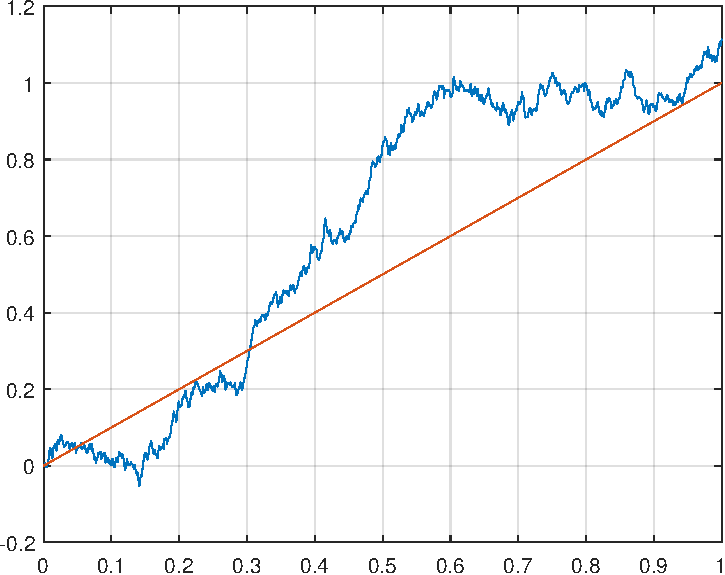
\includegraphics[width=0.5\linewidth]{assets/drift.pdf}
        \caption{Brownian motion with drift}
        \label{fig:drift}
    \end{figure}

    The drift-brownian motion is a gaussian process. To calculate the mean and variance of such process, just take the expected value

    \begin{equation}
        E(X_t) = E(\mu t + \sigma B_t) = \mu t + \sigma E(B_t) = \mu t
    \end{equation}
    \begin{gather}
        Cov(X_s, X_t) = E((\mu t + \sigma B_t)(\mu s + \sigma B_s)) - E(\mu t + \sigma B_t) E(\mu s + \sigma B_s) = \notag \\
        = E(\mu^2 t s + \mu \sigma B_s + \mu \sigma B_t + \sigma^2 B_s B_t) - \mu^2 ts = \notag \\
        = \mu^2 ts + \sigma^2 E(B_s B_t) - \mu^2 st = \sigma^2 (t \wedge s)
    \end{gather}
    \item[Brownian Bridge] Take a real number $0 \leq t \leq 1$ and define $X_t = B_t - tB_1$. It's easy to see that $X_0 = 0$ and $X_1 = 0$. This is also a gaussian process.

    \begin{figure}[h!]
        \centering
        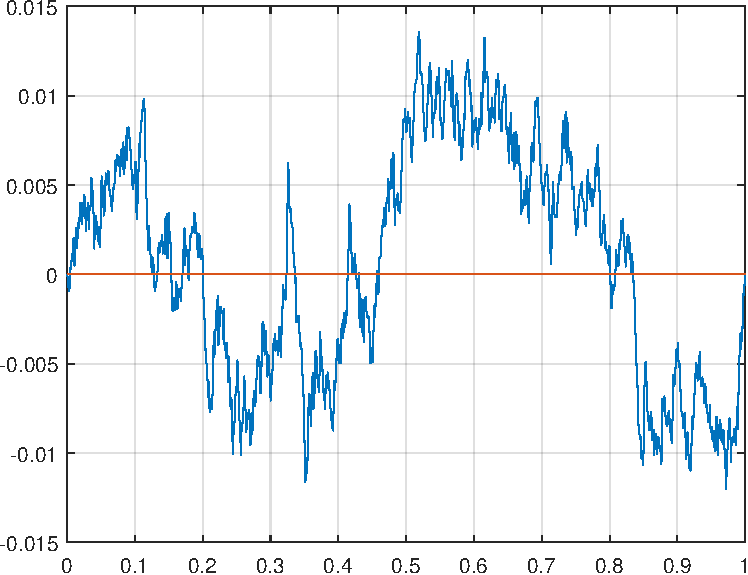
\includegraphics[width=0.5\linewidth]{assets/bridge.pdf}
        \caption{The process shows mean-reversion: the more it gets away from the mean, in this case zero, the quicker it will converge back to it}
        \label{fig:bridge}
    \end{figure}

    \begin{equation}
        E(X_t) = E(B_t - t B_1) = 0
    \end{equation}
    \begin{gather}
        Cov(X_t, X_s) = E(X_t X_s) - E(X_t) E(X_s) = E\big(B_t B_s - t B_1 B_s - s B_1 B_t + ts B_1^2\big) = \notag \\
        = s \wedge t - s \big(t \wedge 1\big) - t \big( s \wedge 1 \big) + ts = s -st -st + st = s(1-t)
    \end{gather}
    where we've assumed $s \leq t \leq 1$. 
    \item[Geometric Brownian Motion] Given a brownian motion $B_t$ and two parameters $\mu \in \mathbb{R}$, $\sigma > 0$ we define the \textit{geometric brownian motion}
    \begin{equation}
        S_t = \exp{\mu t + \sigma B_t}
    \end{equation}
    This process is of fundamental importance in quantitative finance, as the price dynamics of stocks is assumed to behave exactly like this. In particular, $X_t$ is distributed like a lognormal distribution, so that $\log(X_t) \sim \mathcal{N}(\mu t, \sigma^2 t)$. 

    \begin{figure}
        \centering
        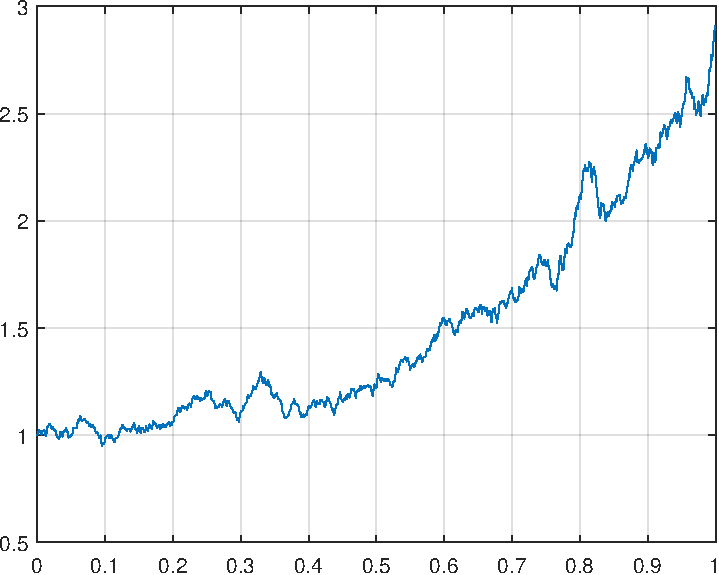
\includegraphics[width=0.5\linewidth]{assets/gbm.pdf}
        \caption{Geometric Brownian Motion}
        \label{fig:gbm}
    \end{figure}
\end{description}

Let's sum up what we have concluded in this section: by use of Kolmogorov existence theorem, we know a brownian motion does exist, with respect to the natural filtration; furthermore, using Kolmogorov continuity theorem, we've that the brownian motion admits a continuous modification. However, the natural filtration is usually not what we work with: we wish the two results above were still true with respect to the \textit{augmented filtration} $\bar{\mathcal{F}} = \sigma(\mathcal{F},\mathcal{N})$. 

\begin{proposition}
    If $B$ is a $\mathcal{F}_t-$brownian motion, then $B$ is also a $\mathcal{F}_{t^+}-$brownian motion, where
    \begin{equation*}
        \mathcal{F}_{t^+} = \bigcap_{\epsilon > 0} \mathcal{F}_{t+\epsilon}
    \end{equation*}
\end{proposition}
\begin{proof}
    Since $B$ is a brownian motion with respect to $\mathcal{F}$, the first two properties $B_0 = 0$ and $B_t-B_s \sim \mathcal{N}(0,t-s)$ are already satisfied. We need to check that the increments are independent $B_t-B_s \indep \mathcal{F}_{s^+}$. This is equivalent to checking that, for every bounded and continuous $h$ the conditinal expectation $E\big(h(B_t-B_s) \vert \mathcal{F}_{s^+} \big) = E\big(h(B_t-B_s) \big)$. Given an intenger $n$, consider
    \begin{gather*}
        B_{t+\frac{1}{n}}-B_{s+\frac{1}{n}} \indep \mathcal{F}_{s+\frac{1}{n}} \supseteq \mathcal{F}_{s^+} \\
        \implies B_{t+\frac{1}{n}}-B_{s+\frac{1}{n}} \indep \mathcal{F}_{s^+}
    \end{gather*}
    We now take the conditional expectation with respect to $\mathcal{F}_{s^+}$ of the function $h$ of the increment, which can be factored out since its independence
    \begin{equation*}
        E\big( h(B_{t+\frac{1}{n}}-B_{s+\frac{1}{n}}) \big\vert \mathcal{F}_{s^+} \big) = E\big( h(B_{t+\frac{1}{n}}-B_{s+\frac{1}{n}}) \big) = E\big(h(B_t-B_s)\big)
    \end{equation*}
    We now take the limit as $n \to \infty$; by the dominated convergence theorem, recall that $h$ is by assumption bounded, we can bring the limit inside of the expectation
    \begin{gather*}
        \lim_{n \to \infty} E\Big( h\big(B_{t+\frac{1}{n}}-B_{s+\frac{1}{n}}  \big) \Big\vert \mathcal{F}_{s^+} \Big) = E\Big( \lim_{n\to\infty} h\big( B_{t+\frac{1}{n}} - B_{s+\frac{1}{n}} \big) \Big\vert \mathcal{F}_{s^+} \Big) = \\
        = E\Big( h\big( B_t - B_s \big) \Big\vert \mathcal{F}_{s^+} \Big) = E\Big( h\big( B_t - B_s \big) \Big)
    \end{gather*}
    Since this holds for every continuous, bounded function $h$, we can conclude that $B_t - B_s \indep \mathcal{F}_{s^+}$. So $B_t$ is indeed a brownian motion with respect to $\mathcal{F}_{s^+}$. 
\end{proof}

\begin{corollary}
    If $B_t$ is a $d-$dimensional $\mathcal{F}_t- $brownian motion, then the same process $B_t$ is also a $\bar{\mathcal{F}}_{t^+}$ brownian motion, where
    \begin{equation*}
        \bar{\mathcal{F}}_{t^+} = \cap_{\epsilon > 0} \bar{\mathcal{F}_{t^+}} \;\; \text{where} \;\; \bar{\mathcal{F}}_{t^+} = \mathcal{F}_{t^+} \vee \mathcal{N}
    \end{equation*}
\end{corollary}

\begin{proposition}
    Given a $d-$dimensional and continuous brownian motion $\big( \Omega, \mathcal{F}, (\mathcal{G}_t)_t, (B_t), \mathbb{P} \big)$, where $\mathcal{G}_t = \sigma(B_s, s \leq t)$ then
    \begin{itemize}
        \item The augmented natural filtration is right continuous, $\bar{\mathcal{G}}_{t} = \bar{\mathcal{G}}_{t^+}$
        \item The tuple $\big( \Omega, \mathcal{F}, (\bar{\mathcal{G}}_t)_t, (B_t), \mathbb{P} \big)$ is a \textit{standard} and continuous brownian motion. In particular, this means that the augmented natural filtration $(\mathcal{G}_t)$ is complete and right-continuous. 
    \end{itemize}
\end{proposition}

\subsection{Poisson Process}
So far, we have considered only \textit{almost surely} continuous processes, like the brownian motion. We now turn ourselves to a process that does not meet this requirements. 

Consider a time interval $[0,T]$, during which some events may happen. We wish to count how many of these happen as time goes by, assuming the following: the intensity of arrivals is constant, multiple arrivals can not happen at the same time, each arrival is independent of each other. 

\begin{definition}
    A stochastic process $(N_t)_t$ is a Poisson process, with rate $\lambda > 0$, if 
    \begin{enumerate}
        \item $N_0 = 0$, $\mathbb{P}-$almost surely
        \item The number of arrivals in disjoint time intervals are independent 
        \item The distribution of the number of arrivals, in a time interval, depends only on the size of the interval, not the starting point
        \item The following limits hold
        \begin{equation*}
            \lim_{h \to 0} \frac{\mathbb{P}(N_h = 1)}{h} = \lambda \;\;\;\;\; \lim_{h \to 0} \frac{\mathbb{P}(N_h \geq 2)}{h} = 0
        \end{equation*}
    \end{enumerate}
\end{definition}

By point $2$, we can conclude that $N_t \indep N_{t+s}-N_t$, for any $t,s$. Moreover, the third hypothesis implies that the distribution $N_{t+s}-N_t$ depends only on $t-s$.

\begin{proposition}
    Let $N_t$ be a Poisson process, with $\lambda > 0$. Then
    \begin{equation}
        \mathbb{P}(N_t = k) = e^{-\lambda t} \frac{(\lambda t )^k}{k!} \;\;\;\;\; k = 0,1,...
    \end{equation}
    In other words, $N_t \sim Po(\lambda t)$. This random variable describes the number of arrivals in the time interval $[0,t]$. 
\end{proposition}

This proposition also serves as another characterization of a Poisson process. In fact, a stochastic process $N_t$ is a Poisson process if 
\begin{itemize}
    \item $N_0 = 0$ almost surely
    \item It's a stationary process with independent increments 
    \item For every $0 \leq s \leq t$, the increments $N_t-N_s \sim \mathcal{P}\big(\lambda(t-s)\big)$
\end{itemize}

Recall that a stationary process if increments $X_{t+h}-X_{s+h} \sim X_t-X_s$. Let's compute the mean and the covariance. 

\begin{gather*}
    E(N_t) = \lambda t \;\;\; Var(N_t) = \lambda t \;\;\; E(N_t^2) = \lambda t+\lambda^2 t^2 \\
    Cov(N_s,N_t) = E(N_t N_s) - E(N_t)E(N_s) = E\Big( (N_t-N_s+N_s) N_s \Big) -\lambda t \lambda s = \\
    = E\Big( (N_t-N_s)N_s \Big)-E(N_s^2)-\lambda^2 ts = \lambda(t-s) \lambda s + \lambda t + \lambda^2 t^2 - \lambda^2 ts = \lambda s \\
    \implies Cov(N_s,N_t) = \lambda (s \wedge t)
\end{gather*}

We see that the rate of Poisson process is equal to the average number of arrivals per unit of time. In general, $\lambda$ may or may not be constant over time, it could also be measurable function of time. 

Consider an interval $[0,t]$, during which $N_t$ arrivals occur. Let $s_i$ be the time the $i-$th arrival happened; this is a sequence of stopping times.  